\section{Background} \label{background}
In this section, we first briefly introduce the background of RDMA and RDMA virtualization techniques.

\subsection{RDMA}
RDMA infrastructure is built for distributed applications that require high-performance and low latency network communications in data centers.
It uses a zero copy approach to deliver data between servers. With RDMA, applications can read and write memory of a remote machine, without the participation of CPU and OS kernel on both sides. Based on these features, RDMA has been adopted to various high-performance distributed systems~\cite{dragojevic2014farm}~\cite{wei2015fast}~\cite{lu2017octopus}, deep learning frameworks~\cite{abadi2016tensorflow}~\cite{chen2015mxnet}, and big data systems~\cite{spark-rdma}~\cite{hadoop-rdma}.

In the workflow of RDMA, the control path and the data path are separated. As shown in Figure~\ref{fig:rdma-feat}, on the control path, the application creates QP(Queue Pair), CQ (Completed Queue), registers MR (Memory Region) and other RDMA metadata, and caches the metadata to RNIC, such as queue ID, MR key, page tables. On the data path, the application can write to  the DoorBell register to notify RNIC of a new request. RNIC will read the request in the QP, read/write the contents of the local/remote MR, and put the completion notifications into the CQ. The application can poll the CQ to get the notifications. The housekeeping work is done on the control path that involves the OS kernel. The performance critical data transmission work on the data path totally bypasses the OS kernel.

RDMA can be implemented in different ways, for example, InfiniBand \cite{infiniband}, Roce \cite{roce}, and iWARP \cite{iwarp}. Verbs library \cite{verbs} provides a basic interface for applications to use RDMA that hides the differences at driver and hardware levels. It is similar to socket layer for traditional network applications. On the control path Verbs provides APIs like ibv\_create\_qp, ibv\_reg\_mr. On the data path Verbs provides APIs like ibv\_post\_send and ibv\_post\_recv.

\begin{figure}[!ht]
	\centering
	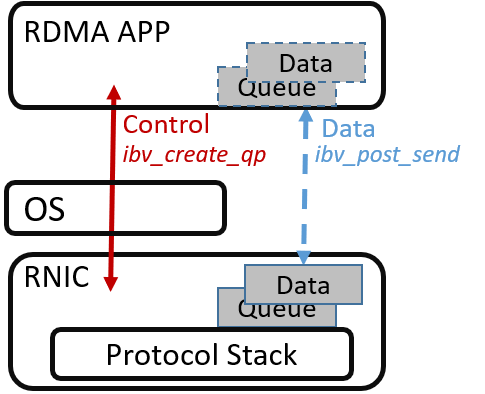
\includegraphics[width=0.8\linewidth]{images/rdma-feat.png}
	\caption{Native RDMA Architecture: the control path and data path are separated}
	\label{fig:rdma-feat}
\end{figure}

\subsection{RDMA Virtualization}
Nowadays, VMs and containers are both common virtualization techniques in data centers.

For virtualizing I/O devices, there are two main choices for where to emulate the device: kernel-space or user-space. In kernel-space, the code of device emulation are inserted into hypervisor or host kernel. Compared to kernel-space, there are three advantages for user-space: first, the attack surface is limited for user-space with minimal inserted code into kernel/hypervisor; second, management logics can be flexibly implemented in user-space; third, the RDMA kernel modules are usually dependent on kernel APIs (e.g. OS architecture, device driver). For example, vhost-net~\cite{vhost-net} is the kernel-space network device and vhost-user-net~\cite{vhost-user-net} has user-mode virtual device.